% $Id: template.tex 11 2007-04-03 22:25:53Z jpeltier $

\documentclass{vgtc}                          % final (conference style)
% \documentclass[review]{vgtc}                 % review
%\documentclass[widereview]{vgtc}             % wide-spaced review
%\documentclass[preprint]{vgtc}               % preprint
%\documentclass[electronic]{vgtc}             % electronic version

%% Uncomment one of the lines above depending on where your paper is
%% in the conference process. ``review'' and ``widereview'' are for review
%% submission, ``preprint'' is for pre-publication, and the final version
%% doesn't use a specific qualifier. Further, ``electronic'' includes
%% hyperreferences for more convenient online viewing.

%% Please use one of the ``review'' options in combination with the
%% assigned online id (see below) ONLY if your paper uses a double blind
%% review process. Some conferences, like IEEE Vis and InfoVis, have NOT
%% in the past.

%% Figures should be in CMYK or Grey scale format, otherwise, colour 
%% shifting may occur during the printing process.

%% it is recomended to use ``\cref{sec:bla}'' instead of ``Fig.~\ref{sec:bla}''
\graphicspath{{figures/}{pictures/}{images/}{./}} % where to search for the images

\usepackage{times}                     % we use Times as the main font
\renewcommand*\ttdefault{txtt}         % a nicer typewriter font

%% Only used in the template examples. You can remove these lines.
\usepackage{tabu}                      % only used for the table example
\usepackage{booktabs}                  % only used for the table example
\usepackage{lipsum}                    % used to generate placeholder text
\usepackage{mwe}                       % used to generate placeholder figures
\usepackage{cite}
\usepackage{amsmath,amssymb,amsfonts}
\usepackage{algorithmic}
\usepackage{graphicx}
\usepackage{textcomp}
% \usepackage{xcolor}
%% We encourage the use of mathptmx for consistent usage of times font
%% throughout the proceedings. However, if you encounter conflicts
%% with other math-related packages, you may want to disable it.
\usepackage{mathptmx}                  % use matching math font


%% If you are submitting a paper to a conference for review with a double
%% blind reviewing process, please replace the value ``0'' below with your
%% OnlineID. Otherwise, you may safely leave it at ``0''.
\onlineid{0}

%% declare the category of your paper, only shown in review mode
\vgtccategory{Research}

%% allow for this line if you want the electronic option to work properly
\vgtcinsertpkg

%% In preprint mode you may define your own headline. If not, the default IEEE copyright message will appear in preprint mode.
%\preprinttext{To appear in an IEEE VGTC sponsored conference.}

%% This adds a link to the version of the paper on IEEEXplore
%% Uncomment this line when you produce a preprint version of the article 
%% after the article receives a DOI for the paper from IEEE
%\ieeedoi{xx.xxxx/TVCG.201x.xxxxxxx}


%% Paper title.

\title{A Hybrid Architecture for Low Latency AR Alignment}

%% This is how authors are specified in the conference style

%% Author and Affiliation (single author).
%%\author{Roy G. Biv\thanks{e-mail: roy.g.biv@aol.com}}
%%\affiliation{\scriptsize Allied Widgets Research}

%% Author and Affiliation (multiple authors with single affiliations).
%%\author{Roy G. Biv\thanks{e-mail: roy.g.biv@aol.com} %
%%\and Ed Grimley\thanks{e-mail:ed.grimley@aol.com} %
%%\and Martha Stewart\thanks{e-mail:martha.stewart@marthastewart.com}}
%%\affiliation{\scriptsize Martha Stewart Enterprises \\ Microsoft Research}

%% Author and Affiliation (multiple authors with multiple affiliations)
\author{Roy G. Biv\thanks{e-mail: roy.g.biv@aol.com}\\ %
        \scriptsize Starbucks Research %
\and Ed Grimley\thanks{e-mail: ed.grimley@aol.com}\\ %
     \scriptsize Grimley Widgets, Inc. %
\and Martha Stewart\thanks{e-mail: martha.stewart@marthastewart.com}\\ %
     \parbox{1.4in}{\scriptsize \centering Martha Stewart Enterprises \\ Microsoft Research}}

\author{Matthew Desaulniers and Qi Han\\ 
Department of Computer Science \\
Colorado School of Mines, Golden, CO, USA \\
\{mdesaulniers,qhan\}@mines.edu}

%% A teaser figure can be included as follows
% \teaser{
%   \centering
%   
\includegraphics[width=\linewidth]{CypressView}
%   \caption{In the Clouds: Vancouver from Cypress Mountain.}
%   \label{fig:teaser}
% }

%%%%%%%%%%%%%%%%%%%%%%%%%%%%%%%%%%%%%%%%%%%%%%%%%%%%%%%%%%%%%%%%%%%%
%%%%%%%%%%%%%%%%%%%%%%% Reviewer Notes %%%%%%%%%%%%%%%%%%%%%%%%%%%%%
%%%%%%%%%%%%%%%%%%%%%%%%%%%%%%%%%%%%%%%%%%%%%%%%%%%%%%%%%%%%%%%%%%%%

%%%%%%%%%%%%%%%%%%%%%%%% Reviewer 1 %%%%%%%%%%%%%%%%%%%%%%%%%%%%%%%%

% 1. ✅Index terms should be in alphabetical order
% 2. ✅Some missing descriptions towards the end of Figure 2 need to 
    % be clarified (more specifically, what happens towards the end 
    % of the flow of the proposed framework).
% 3. ✅Add missing citations for claims referring to the existing 
    % body of knowledge and term definitions.

%%%%%%%%%%%%%%%%%%%%%%%% Reviewer 2 %%%%%%%%%%%%%%%%%%%%%%%%%%%%%%%%

% 1. Future work should focus on two areas: the scalability of the 
    % concept (as already mentioned by the authors), and the 
    % investigation of different and asymmetric network performance 
    % categories for the second step. For example, what happens if 
    % some users are on the same local network (with short delays) 
    % while others experience long delays, inevitable due to 
    % wide-area network transport?

%%%%%%%%%%%%%%%%%%%%%%%% Reviewer 3 %%%%%%%%%%%%%%%%%%%%%%%%%%%%%%%%

% 1. ✅As the experiment conducted was limited to three devices only, 
    % the benefits/impacts of peer-to-peer information exchange may 
    % be different for scenarios with more devices (causing higher 
    % local latency on the network and more computational efforts 
    % to align the n different point clouds). This might, at some 
    % point, be overcome by means of utilizing multicast or 
    % broadcast network technologies rather than collisin-prone 
    % point-to-point communication, which would have been great to 
    % see addressed or at least discussed in this work as well.

% 2. Also, I wonder on the robustness of the approach towards rapid 
    % motion of objects. The example scenario discussed does not only 
    % require low latency, but also has high dynamics in the AR object 
    % position and relocation aspects (as in: high speed of objects), 
    % potentially negatively impacting on the validity, quality, or 
    % computational complexity of the described approach. This could 
    % have been addressed more precisely in the paper.

%%%%%%%%%%%%%%%%%%%%%%%%%%%%%%%%%%%%%%%%%%%%%%%%%%%%%%%%%%%%%%%%%%%%

%% Abstract section.
\abstract{
  Multi-user Augmented Reality (AR) systems are critical for the enhancement of existing and future collaborative 
  robotic systems. Multi-user systems provide information that may otherwise be unavailable to an independent user 
  and augmented reality enables the integration of that information naturally into the human perception system. Multi-user AR 
  systems can scale large, become complex, and generate quantities of data that must be managed and communicated 
  between users. This paper describes efforts to lower human perceived end-to-end latency of a multi-user AR system.  The system is measured with respect to user perceived latency as a motivation for directing efforts for future system-level research 
  as well as improvements. We find that the latency bottleneck is associated with the cloud server based user alignment 
  system.
   
  We augment the system with a peer-to-peer alignment scheme that runs in parallel to the cloud server based alignment. We 
  implement the new user alignment system and measure latency and user alignment accuracy with respect to the user expected cloud server alignment. 
  Finally we analyze data from experiments conducted with the fully implemented system. We find that the peer-to-peer hybrid
  system along with our proposed gravity-based alignment drastically reduces user perceived latency at the cost of some variance in positional and angular accuracy. We 
  discuss future work on how the system may be made more robust to scaling and network conditions. 
} % end of abstract

%% Keywords that describe your work. Will show as 'Index Terms' in journal
%% please capitalize first letter and insert punctuation after last keyword.
\keywords{Alignment, Augmented Reality, Point Registration.}

%% Copyright space is enabled by default as required by guidelines.
%% It is disabled by the 'review' option or via the following command:
% \nocopyrightspace

%%%%%%%%%%%%%%%%%%%%%%%%%%%%%%%%%%%%%%%%%%%%%%%%%%%%%%%%%%%%%%%%
%%%%%%%%%%%%%%%%%%%%%% START OF THE PAPER %%%%%%%%%%%%%%%%%%%%%%
%%%%%%%%%%%%%%%%%%%%%%%%%%%%%%%%%%%%%%%%%%%%%%%%%%%%%%%%%%%%%%%%%

\begin{document}

%% The ``\maketitle'' command must be the first command after the
%% ``\begin{document}'' command. It prepares and prints the title block.

%% the only exception to this rule is the \firstsection command
\firstsection{Introduction}

\maketitle

%% \section{Introduction} %for journal use above \firstsection{..} instead
% Focus the introduction on low latency. Why latency is important

As AR technology advances, its uses will expand into real-time applications. Scenarios like 
emergency response, surgical procedures, piloting aircraft, and vehicle operation will require extremely low latency 
in order to be considered feasible application spaces. 

A promising benefit of these systems is the ability for more cohesive collaboration between humans and robots. A great advantage 
of human-robot collaboration is the ability to combine the the high-level decision making of a human along with the deep level of 
information that may be provided by sensors accessible to machines. One such application is for users to see occluded objects in 
real-time. For instance, suppose a warehouse forklift operator is navigating through 
aisles in a warehouse. There is no way of knowing if there may be another person or vehicle coming around any given corner
without some form of secondary information besides auditory or basic visual cues. In this scenario, where a warehouse 
is already filled with modern sensors, like cameras, the perception ability of the forklift operator may be augmented 
by the warehouse sensor suite itself. Upon reaching an occluded turn, the operator is automatically given ``line of sight" 
via rendered representations of people or obstacles that could not otherwise be seen. The process of giving a vehicle operator 
enough time to perceive and react to an incoming obstacle/person requires any solution to adhere to 
real-time latency constraints. This system is completely dependent 
on users having a shared reference frame such that obstacles appear where they would in the real world to give the user
a sense of ``line of sight" and must function with latency requirements on the scale of human
reaction time. 

These applications lend themselves to effectively extending the sensory abilities
and perception of a user and so demand comparable latency to that of human reaction and sensing times. 
Achieving object placement and user to user alignment accurate enough for critical applications (cm to sub-cm scale) % TODO May need a citation for this 
and strict adherence to low-latency requirements necessitate demanding design constraints for AR devices. 


%  Why latency is challenging

Achieving low latency in an AR system provides a unique challenge due to the applications in which it may be applied.
From a technical perspective, many of the components that make up the system (SLAM, alignment, modeling, etc.) are 
well developed in their fields. These components work well on performance computing systems, but represent a 
challenge when the practical aspects of AR systems are applied.
By nature of AR being a method of directly interacting with the 
world around a user, an AR system must be portable and small in size, whether with respect to vehicle or human. Not only must 
it be small in form factor, but it should also have high computational ability. These factors result in 
high cost for devices that render AR solutions infeasible within many application spaces. As in our previous warehouse scenario, the close 
proximity between the operator and object/person of interest requires the system to function at real-time latencies. This work
aims to decrease end-to-end system latency without significantly sacrificing object placement accuracy using common off-the-shelf AR devices for users in close proximity. 

% This reduced size for portability demands a direct trade-off between system size and cost as a consequence. A system that is portable and can
% successfully compute spatial/visual computations for AR independently would be therefore prohibitively costly. This 
% cost would render AR infeasible for many applications. Low latency requirements are particularly opposed to AR 
% user design fundamentals. 

%  What has been done so far
There are multiple perspectives in which this problem has been approached by the multi-user AR research community \cite{BreakingEdgeShackles,hambazi,AdaptSLAM,SEESys}.
Many works solve this trade-off between system cost and computational ability by offloading compute to edge or 
cloud servers. This decreases the local  costs of computation on a user device, but increases 
total system complexity by introducing a network component and latency associated with network routing and 
physical distance between user and server. Conversely, some systems implement peer-to-peer solutions that take advantage 
of the close proximity of users to cooperatively attain better solutions or remove redundant calculations.
Given the multi-faceted nature of AR systems, there are a number of research areas that have seen efforts to improve
multi-user latency for streaming \cite{intelli-ar}, SLAM \cite{SLAMShare}, object detection \cite{SEAR}\cite{Nimbus}, 
and view alignment \cite{communication-efficient-spatially-consistent}\cite{ARLight}. For most state-of-the-art approaches, researchers
tend to exclusively design either client-server based offloading systems or peer-to-peer systems. There is a much smaller 
subset of works that create hybrid systems utilizing a client-server model as well as a peer-to-peer component. These 
tend to lower end-to-end latency\cite{SCAXR}\cite{SEAR}. 

% TODO Cite HERE

% What's your approach. This is where maybe contributions are listed.
User alignment is a fundamental component of multi-user AR systems. Alignment ensures that users may interact with each other in a way that is spatially consistent across a group. 
User alignment is the process of finding the transformation between user reference frames such that we may correctly place objects in the same real-world position with 
respect to all users. An improperly aligned world view would result in one user seeing an object in a different position or orientation from another user. This is an essential, and often first, step that comes at 
the high cost of end-to-end system latency due to cloud servers having long network delay and latency due to computational overhead. 
We have set out to improve the peer-to-peer alignment latency of a cloud-based alignment anchor system. Our system creates a peer-to-peer alignment method that augments the existing client-server model. This new hybrid architecture 
will enable real time alignment that becomes more stable and consistent across sessions as the cloud server resolves its solution. 
The specific major contributions of this work are as follows. 
\begin{itemize}
    \item We have conducted an exploratory study on end-to-end latency of current solutions for user interactions and the data flow in multi-user AR 
    of resource-constrained devices. This study led us to address the latency bottleneck in the cloud-based alignment process. 
    \item We have implemented a hybrid architecture for multi-user AR that combines a client-server model and a peer-to-peer model using Android phones.
    \item We have developed a gravity-based user alignment approach that is able to resolve alignment in resource-constrained mobile devices.  % an order of magnitude faster than cloud-based methods 
    \item We have compared the end-to-end latency of our system against a common cloud solution using Google Cloud servers. This 
    resulted in reductions from over 3000ms to approximately 100ms at the expense of cm scale anchor jitter.
\end{itemize}

\section{Related Work}

User alignment in AR is generally accomplished 
in two ways. 

First, alignment may be achieved as a byproduct of computing SLAM algorithms and communicating 
information relating to user maps \cite{decentralized-slam}. This often 
involves either allowing an edge computer to host the centralized SLAM map, rendering the users dependent on the 
edge computer or allowing users to share maps between themselves, which can lead to complexity with keyframe selection
and sending reduced size maps. SLAMShare\cite{SLAMShare} utilizes a nearby edge server to provide consistency for serving a hosted 
map to a group of users as well as reduced latency time from computational overhead. This drastically improves latency, but 
creates no method for alignment when an edge server is unavailable. FreeAR \cite{BreakingEdgeShackles} effectively turns a 
peer-to-peer system into a client-server relationship, by electing one user to conduct all SLAM calculations for the group. 
The elected host device receives updates from peers and returns the peer position in its map. While this reduces some latency
in the form of time taken to synchronize maps, the alignment is still only as accurate as a the ability of a mobile device will allow.

The second method is through direct user to user alignment. This has been achieved a number of ways. 
The concept of sending keyframes is a recurring theme in these works. A keyframe may be defined as a frame within a 
sequence of spatial data (this may be video or point clouds) that is chosen as a particularly useful frame \cite{BreakingEdgeShackles}. Usefulness may 
be due to a particularly rich feature set or the timing of the frame itself with respect to the system processes. In some cases,
the keyframe is 3D data that is compressed back into a 2D data structure, like an image, and sent as if it were a feature-rich 
image frame\cite{ARLight}. Alternatively, some have used the keyframes generated from SLAM to begin a separate alignment process \cite{communication-efficient-spatially-consistent}.
As SLAM keyframes are generated, they are selectively saved off until a number of keyframes have been accumulated. This is then
sent as a message to peers to resolve. Keyframes are chosen by proximity to an object of interest that a host wishes 
peers to resolve with respect to. 

All direct alignment works were found to be peer-to-peer based and works using SLAM to begin with were split between
peer-to-peer and client-server based architectures. While these all lowered system latency in some way, the works 
that created peer-to-peer systems were left with systems that were not as accurate as client-server models and client-server models 
suffer from either network delay or leave no explanation for how latency may be affected when the server is unavailable.

SEAR \cite{SEAR} utilizes an architecture for object detection for multi-user AR that allows the system to take advantage of 
both peer-to-peer and client-server models. As in the previous server-based approaches, users may request object detection tasks 
from the edge server. In many cases the server will comply and return a result. Upon receiving the result the user 
will cache the response. As other users make requests, the server may deny a request. If this happens, users will request 
their peers to resolve it. All peers then check their caches and return the result if found. While SEAR simply brings 
two simple architectures together, it results in a massive gain for multi-user object detection. Likewise, SCAXR \cite{SCAXR}
implements a similar tiered architecture. An edge computer is assigned as the scheduler and this computer then monitors 
server resource use vs computational ability of users. If the scheduler needs to create room for server usage, it may direct a 
request to another user. The SCAXR system greatly improved rendering task latency for multi-user AR systems. 

% While there exists peer-to-peer alignment systems and client-server based alignment systems, there is no hybrid architecture 
% alignment system that takes advantage of the speed of peer-to-peer solutions and accuracy of server-based solutions.



{\it While there exist peer-to-peer alignment systems and client-server based alignment systems, there exists no hybrid architecture 
alignment systems that take advantage of the speed of peer-to-peer solutions and accuracy of server-based solutions.}

\section{Exploratory Studies}
The purpose of this exploratory study is two-fold. The implementation of a multi-user AR application will yield a 
framework that can be used to evaluate existing AR features/algorithms and to identify aspects within these 
applications that may present themselves as weak points in current multi-user AR systems.

We implemented a multi-user AR system using three Google 
Pixel 5 smartphones. Each phone contains a Snapdragon 765G processor and 8GB of RAM. They are running on the Android 14 operating 
system. This model phone does not have LiDAR, but uses dual cameras for depth sensing. All three phones operate on the same local network.

We implemented a simple AR application where users make basic commands (i.e. place object, resolve cloud anchors, and host cloud anchors) 
that are propagated to other devices. The system is made up of user devices that are all peers, able to freely send
information between themselves, and a cloud server. The role of the cloud server is to allow the users to conduct accurate world alignment between 
their respective reference frames. The cloud server hosts the original data used by a host user device to initiate an alignment as well as executes 
an alignment algorithm for any user that may request it. A host user device is simply the peer that initiates that request to host a cloud anchor 
and sends the  cloud anchor ID to its peers. Peer devices that receive the ID and query the cloud server are referred to as a resolver device. Once 
user alignment is achieved, user devices may automatically recognize objects/images of interest in their environment and send their location to their peers. 
Those peers will then use the cloud-based alignment system to place those objects accurately within their own reference frame. The alignment allows users to 
place objects that other users will automatically see in a way that is spatially consistent. If some user places in object in a shared 
space, then all other users in the space will see the object where that user placed it. 

% We implemented a simple AR application where users make basic commands (i.e., place object, resolve cloud anchors, and host cloud anchors) 
% that are propagated to other devices (world 
% alignment), peer user devices 
% automatically detect images in their surroundings and place objects in their own and other user's view, and create 
% a visualization of a generated world map. In short, this allows users to place objects that other users will automatically see in a way 
% that is spatially consistent. If some user places in object in a shared space, then all other users in the space will see the object 
% where that user placed it. 

 Application development was conducted in the widely-used Unity game development 
platform and AR-specific functions were built from AR Foundation and ARCore libraries. We used
Google's cloud-based Cloud Anchor alignment system. UDP sockets were used for communication between peer devices and the ARCore 
API was used for making requests to Google Cloud servers. 
This application consists of several major components: SLAM, object detection, streaming and peer-to-peer communication, and alignment. We measured the latencies incurred by these components and show the results in Table \ref{tab:baseline}. 
\begin{table}[!htb]
    \centering
    \begin{tabular}{|l|r|}
        \hline
        Process & Time (ms) \\
        \hline \hline
        Hosting Cloud Anchor ($t_{host}$) & 3,725 \\
         \hline
        Host sends anchor ID to peers & 6.2 \\
        \hline
        Peer Receives Anchor ID & 3.5\\
        \hline
        Peer resolves Cloud Anchor ($t_{resolve}$) & 728\\
        \hline
        User communications AR object to peers  & 9.2\\
        \hline
        Peer places object locally & 1.05\\
        \hline
    \end{tabular}
    \caption{Latency breakdown of Google's cloud-based Cloud Anchor alignment system.}
    \label{tab:baseline}
\end{table}


We first observe that the actual placement of objects takes a trivial amount of time (approximately 1ms). Any communication related processes also 
are low latency tasks, as every peer has connectivity to every other peer. We further observe that Hosting Cloud Anchor and Peer Resolves Cloud Anchor items are by far the largest latency bottleneck in the system. These processes are the 
points where a user has made a request to create an anchor that may be used for user alignment and when peer users try to resolve that alignment 
respectively. Given this massive disparity between user alignment latency and other functions, we believe the greatest benefits to user-perceived
system latency is to reduce the latency of the cloud-based alignment system.

Figure \ref{fig:parallelProcessBenchmark} shows a more 
detailed view of the hosting and resolving process between the cloud server and users.
\begin{figure}[!htb]
    \centering
    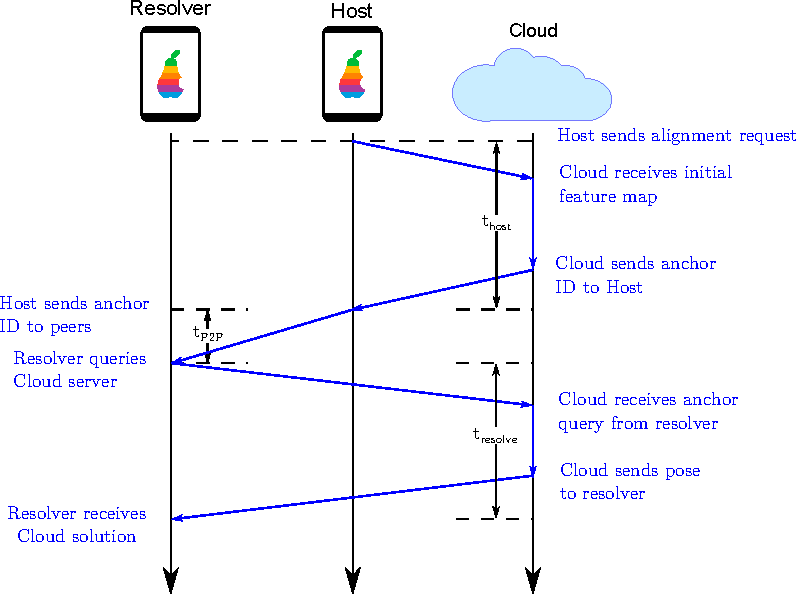
\includegraphics[width=0.5\textwidth]{figure/benchmarkParallel.pdf}
    \caption{Anchor hosting and resolving in Google's cloud-based Cloud Anchor alignment system}
    \label{fig:parallelProcessBenchmark}
    \end{figure}

% In the simplest terms, the baseline system allows users to colocate themselves with respect to an identified 
% point in the real world (1 to n)(n to 1), identify images, place objects, and communicate the location of either identified images
% or placed objects so that other users may place AR objects accordingly. Users may broadcast the location of placed 
% objects to all other users in the network \textbf(Clarify: This action amounts to n to n) (1 to n) or users may request objects from users in the network (n to 1). Latency analysis is completed at the application
% layer of the system. Timing is measured with respect to high level functions that are necessary to the basic operation
% of the system. Conversely, a more comprehensive analysis would take an embedded-level approach to measuring latency across 
% the hardware and lower level software of the android system, but that is outside the scope of this paper.

% Below is a preliminary view of latency analysis for a basic 1-to-1 full system experiment.

% As can be seen in the table, the overwhelming source of latency is the time it takes to request a host anchor or resolve a 
% host anchor with the cloud server. This is due to the computation needed for the cloud server to reliably resolve spatial data 
% from a sequence of video frames as well as the geographical distance between user and cloud server. Another point not necessarily 
% communicated by the latency data is network reliability. Data collected in these experiments was only counted if there was a 
% successful resolve, however there were many instances wherein the server failed to host point clouds due to network issues. 
% The over five second latency above describes the far and away best case for a user that is attempting to host an interaction. 
% Figure \ref{fig:parallelProcessBenchmark} below shows the basic interaction between users and cloud server to host an anchor.

%%%%%%%%%%%%%%%%%%%%%%%%%%%%%%%%%%%%%%%%%%%%%%%%%%%%%%%%%%%%%%%%%%%%%%%%%%%%%%%%%%%%%%%%%%%%%%%%%%%%%%%%%%%%%%%%%%%%%%%%%%%%%%%%%%%%%%%%%%%%%%%%%%%%%%%%




\section{Our Approaches}
To achieve a system that provides users with real-time alignment, we propose two distinct approaches. The first is a hybrid architecture that uses peer-to-peer results to supply an almost instant user alignment which is then replaced by a higher latency, but
more accurate cloud-based alignment. The second is a gravity constrained  point cloud alignment algorithm that runs extremely fast on resource-constrained user devices.
The hybrid architecture allows for the cloud-based alignment to be computed in parallel to the peer-to-peer
user alignment system. While the host is awaiting an alignment ID from the cloud server, it begins streaming the associated point cloud of 
the cloud anchor location as well as its gravity vector to resolver user devices. The streamed point cloud is sparse, 50-200 points 
local to the selected location, so that the network and computationally latency may be minimized. Resolvers then take the gravity vector of both devices 
into account to run a user alignment algorithm at periodic intervals to generate new peer-to-peer alignment estimates. 

With this augmentation the overall system adds no new devices, but now the host and resolver devices have 
additional functionality. The host device, upon initiation of a request to the cloud server, now begins streaming its point cloud view to 
resolver devices. Resolver devices receive point clouds from the host to execute a local alignment algorithm until a cloud anchor ID is 
received from the host that the resolver may use to query the cloud server.


% The entire system is defined by three types of devices. 1) The cloud server is responsible 
% for hosting cloud anchors that may be created by a host device and requested by a resolving device. The cloud server is the only 
% device that is not a user device. User devices are either a host device or a resolver device. 2) The host device is a user device 
% that initiates the request for a cloud anchor with the cloud server and also streams its point cloud view to resolver devices. 3) Resolver 
% devices receive point clouds from the host to execute a local alignment algorithm until a cloud anchor ID is received from the host 
% that the resolver may use to query the cloud server. 


%By running this algorithm in parallel, the same system used for exploratory studies may now facilitate user interaction within approximately 100ms. 
% Eventually, the host gets a return UUID from the cloud server that is sent to the resolver peers. The peer devices then 
% send the UUID along with their own video frames to the cloud to achieve a more precise alignment. Upon completing cloud
% alignment, resolvers message the host to be removed from the streaming list.

\subsection{Hybrid Architecture}


The hybrid architecture may be viewed as a system that is accomplished by splitting up the user alignment into two steps. Once an alignment request 
with the cloud server is initiated by the host, the peer group first executes user alignment via peer-to-peer streaming of the host's point cloud to the resolvers. 
This is followed by the second step wherein the cloud server has responded to the request and peer users begin using the cloud-based user alignment 
solution.

To initiate an alignment request the host selects an area they would like to create as a reference point to communicate for peer alignment. Upon
selection, the reference point and video frames are sent to a cloud server so a map of visual features (edges, corners, etc) 
may be created and hosted within the server to define the user requested reference point. This cloud request takes time to propagate through the network, be 
resolved, and return a lookup ID for the host to distribute to resolvers. After the host has selected the reference frame and awaits a response from the cloud 
server, it then begins to stream a lightweight point cloud to its peers with period $t_{streaming}$. 

This presents a technical dilemma: when a user receives point cloud data in a peer-to-peer manner, how do they know 
whether their user alignment was accurate enough? Given the users are trying to establish a shared reference point, 
there is no method of doing this without human intervention or a previous reference point. In order to keep the 
application automated and experience immersive, a device cannot simply trust one point cloud alignment. One might conceivably
allow for enough computation time that an accurate solution is guaranteed, but this would no longer satisfy low latency 
requirements. For this reason, point clouds are streamed at an interval such that resolvers may have opportunities 
to replace erroneous point cloud alignments when they come in. 

This process is detailed in Figure \ref{fig:parallelProcess} below.

\begin{figure}[h]
    \centering
    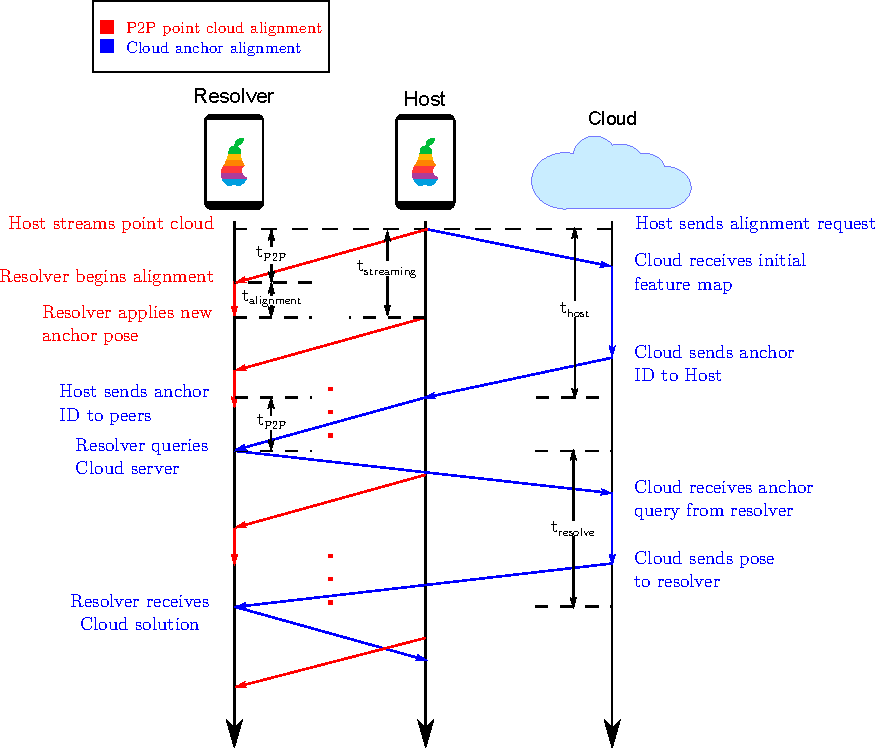
\includegraphics[width=0.5\textwidth]{figure/parallelProcess.pdf}
    \caption{Our hybrid architecture. The sequence of peer-to-peer streamed point cloud messages are shown in red, and the cloud-based alignment is shown in blue. The 
    peer-to-peer streamed messaged are sent periodically by the Host device until the Resolver receives Cloud solution and sends confirmation to the Host.}
    \label{fig:parallelProcess}
\end{figure}



% The chosen approach for improving this latency is by creating a hybrid peer-to-peer/client-server architecture that takes
% advantages from each architecture paradigm. In the traditional client-server model, the users interact with the cloud server to 
% achieve high accuracy user alignment that is extremely stable. This stability comes at the cost of latency and network overhead described 
% in the previous sections as well as network unreliability that comes with interacting with a server that is geographically distant. 
% In a peer-to-peer framework, devices may establish localization extremely quickly with respect to each other. While the localization 
% can be much faster, care must be taken so as not to overwhelm the computational ability of the user device. Further, user devices may 
% drop in and out of an interaction session, but the cloud server will more often than not be available to query for user alignment tasks. 

% Due to the nature of colocating devices with low computational overhead, one cannot guarantee that the point cloud will be perfectly aligned. 
% This presents a technical dilemma: when a user receives point cloud data in a p2p manner, how do they know whether their user alignment was 
% accurate enough? Given the users are trying to establish a shared reference point, there is no method of doing this without human intervention. 
% In order to keep the application automated and experience immersive, a device cannot simply trust one point cloud alignment without taking 
% so long to process it that it becomes equivalent to a cloud server query.

\subsection{Gravity-Based Alignment}


Although AR devices are generally resource-constrained, they often are equipped with a suite of sensors that may be used 
to compensate for a lack of pure computational power. Specifically, IMU modules are ubiquitous in mobile devices and head mounted displays (HMD). By taking 
advantage of the IMU's ability to measure earth's gravity, we reduce the dimensions of the solution space from six to four. 
The peer-to-peer point registration algorithm uses a gravity-based user alignment strategy that can be broken up into three phases:
pre-processing, finding an initial homogenous transformation guess, and finally using this as a starting point for an iterative closest point 
solver. Although all three phases are critical to finding an alignment between users, the use of a gravity vector is particularly unique 
to the system hardware and use case. 

In summary, each peer filters their own point clouds and uses a gravity-based user alignment algorithm to select an initial 
estimate for an iterative closest point (ICP) algorithm. After a transform between point clouds is acquired, the 
views are aligned between host and resolver. This peer-to-peer process is periodically repeated. There is a balance 
to be found in designing this system between accuracy of resolve and $t_{alignment}$. $t_{alignment}$ cannot be so 
short that accuracy is unusable, yet also cannot be so long that it does not significantly improve the user perceived 
latency of the system. This balance must be met by satisfying the requirements demanded by our use case. This system must be able to provide 
input for humans and so should be responsive within approximately human reaction time, which is approximately 100ms \cite{MARVEL}.


{\bf Phase 1. Pre-processing: }
Our pre-processing steps were designed with our specific use case in mind. In this scenario, we 
have a group of users that are known to be within close proximity to each other. Not only do they share close proximity, but we also have some 
notion of group attention. Low latency would not be a requirement if the group was not trying to interact with some common point in space. We may 
use this information to filter out information outside of this shared point of interest (this will be the location of the alignment anchor). 
The resolving devices first conduct frustum culling to remove points outside of their view and a distance based filter that removes points 
that are outside of reasonable interaction distance from the viewer. The final step in preprocessing is gravity alignment. 

A gravity vector is generated using the onboard IMU % Should i go run the math for expected movement limitations and sampling rate of snapdragon imu?
and filtered with a low pass filter,

\begin{equation}
    g_{n+1} = (1-a)g_{n} + a\hat{g}_{n}
\end{equation}

% or,

% % Do we care about this if i don't make a frequency based decision?
% \begin{equation}
%     \frac{G(z)}{\hat{G}(z)} = \frac{a}{1-(1-a)z^{-1}}
% \end{equation}

Where $g_n$ is the estimated gravity vector at time step $n$ and $\hat{g}_n$ is the accelerometer measurement at time $n$. Creating this estimate 
of gravity vectors allows the system to solve for the quaternion responsible for pitch and roll rotations from the host space to the resolver space.

This yields a new quaternion rotation from the resolver reference frame to host reference frame ${}^H\textbf{q}_R$. Let the set of points defining the point cloud of the host and 
resolver be defined as such,

\begin{equation}
{}^RP^R = \{{}^R\textbf{p}^{R}_i \in \mathbb{R}^3 | i = 0, 1, ..., n\}
\end{equation}

\begin{equation}
    {}^HP^H = \{{}^H\textbf{p}^{H}_j \in \mathbb{R}^3 | j = 0, 1, ..., m\}
\end{equation}

Where ${}^HP^H$ is the point cloud received from the Host device in the host reference frame and ${}^RP^R$ is the point cloud in the 
Resolving device reference frame. This rotation is then applied to the resolver point cloud,

\begin{equation}
{}^HP^{R} = \{ {}^H\textbf{q}_R (0, {}^R\textbf{p}^R){}^H\textbf{q}_R^* | {}^R\textbf{p}^R \in {}^RP^R\}
\end{equation}

% The quaternion is used to rotate every preprocessed point before delivering both point clouds the the RANSAC solver.
% The RANSAC algorithm now only must create an initial guess for the 4DOF $(x,y,z,\psi)$. 

{\bf Phase 2: Initial Guess}
Our alignment system now has determined the roll and pitch angles between the host and resolver point clouds. Now that both point clouds 
are in the Host reference frame, the Resolver will run a 4DOF Random Sample Consensus (RANSAC) algorithm to find an initial guess at correspondences
as well as Singular Value Decomposition (SVD) to find the initial transformation guess. RANSAC is a randomized algorithm commonly used for finding good fits 
for data points that is robust to outliers. RANSAC takes a small, sample of each data set, calculates some transformation between the two, and counts the number 
of inlier data points using this transformation. This process is repeated and the transformation with the largest number of inliers is chosen. The choice 
of transformation in our case is guided by physically rotating the point clouds in space and for that reason, SVD is a practical choice.

SVD is a method of calculating correlation of points in a dataset. Specifically SVD provides eigenvectors that represent the major and minor axes 
upon which the dataset it oriented. By creating a covariance matrix between RANSAC sample guesses, we may generate transformations 
that correlate (or physically align) the sample points in space. It is important to note that the SVD calculation blindly assumes that the point clouds 
have the same mean, so this implementation is sensitive to the success of preprocessing assumptions. 

 The initial guess that will be given to the ICP algorithm needs a yaw ($\psi$) value and position vector. This is generated by running a 4DOF RANSAC algorithm that matches linear features. 

The overall execution of RANSAC will follow the traditional method \cite{RANSAC}. The goal of creating the initial guess is to find the best location in 
the ($\psi$, x, y, z) search space that will allow the ICP algorithm to find the optimal alignment without getting stuck in a locally optimal solution. Due to 
the use of lightweight point clouds for fast computation, RANSAC must operate on a sparse feature set of approximately 25-100 $\frac{points}{m^2}$. This is a 
small RANSAC search space (40,000 possible correspondences) by many standards, but still an order of magnitude too large to rely on traditional point to point 
comparisons by constrained user devices.

To ensure good correspondences, we elect to compare visual features. In order to select candidate RANSAC features, the system selects 
two points to create a distance feature found in the data. This feature is the distance between two points such that it is larger than some threshold to 
avoid large yaw error. The resolver choose two points,

\begin{equation}
    |{}^H\textbf{p}^{R}_i - {}^H\textbf{p}^{R}_j| = d^R_{ij} < d_{threshold}
\end{equation}

Once a linear distance feature is found to satisfy this constraint it is used to find a corresponding feature in the host data set such that the features 
are the same distance within some small error.

\begin{equation}
    |{}^H\textbf{p}^{H}_i - {}^H\textbf{p}^{H}_j| = d^R_{ij} < d_{threshold}
\end{equation}

\begin{equation}
    |d^R_{ij} - d^H_{ij}| < d_{error}
\end{equation}


If this constraint is satisfied then the algorithm assumes a match and the traditional inlier count and SVD solution is executed to find an initial guess 
of the 4DOF transformation is returned.

{\bf Phase 3: Transformation Solver}

Solving for the transformation is accomplished by running an ICP solver\cite{simpleICP}. This is accomplished using a simple closest point correspondence 
metric such that points are paired with their nearest neighbors such that they are no greater than 10cm away to filter out outliers. Due to the 
preprocessing and initial guess steps completed, we expect that the ICP algorithm will be provided with point clouds with parallel x-z planes and similar 
centers of mass that only need to be translated and rotated about the y axis. This will allow the algorithm solution to iteratively find the local minima near the 
initial guess. %Running ICP has a complexity of $O(n^2)$ due to the reliance on checking each point to every other point for nearest neighbors. % Don't forget to comment on the kd-tree fix later.

\section{Performance Evaluation}\label{ExperimentalResults}

Experiments were conducted in a variety of well-lit indoor environments. We used the same devices and experimental setup as in our exploratory studies.  To compare the performance between our proposed system and the benchmark system, we consider two metrics. In addition to latency of alignment, we also compare the spatial accuracy of alignment. In this study, we use the accuracy provided by the cloud-based system as the ground truth and measure the error of our system from that. 

\paragraph{\bf Alignment Latency.}
The system begins streaming 
once the host device makes a request query to the cloud server and is awaiting a response. We 
find that the average latency is 119.69ms for each peer-to-peer user alignment. This effectively 
reduces the user perceived latency of the multi-user system from 3.725 seconds to 119.69ms or an approximate 97\% reduction in latency. Table 
\ref{tab:parallel_latency} shows the functions of the benchmark system now including the parallel host transmission of point cloud 
data and resolver time. To gather results, 34 requests to host a cloud anchor were made to the Google cloud server that 
resulted in 392 peer-to-peer user alignment calculations. Network conditions and varying wait times for the response from 
the Google cloud server means that the number of user alignments per hosting event is variable. The average 
number of alignments per host event is 11.5. %I would like to make a graph for this also.


% \begin{center}
%     \begin{tabular}{ |c|c| } 
%      \hline
%      Event & Time (s) \\
%      \hline \hline
%      Cloud Server solves localization &  3725ms \\ 
%      \hline
%      User sends new anchor ID to peers &   \\ 
%      \hline
%      Peer receives anchor ID&   \\ 
%      \hline
%      Cloud server resolves anchor&   \\ 
%      \hline
%      User detects image &   \\ 
%      \hline
%      User places object &   \\ 
%      \hline
%      User communicates object to peers &   \\ 
%      \hline
%      Peer places object locally&   \\ 
%      \hline
%      RTT ping &   6ms\\ 
%      \hline
%     \end{tabular}
% \end{center}


\begin{table}[!htb]
    \centering
    \begin{tabular}{|l|r|}
        \hline
        Process & Time (ms) \\
        \hline \hline
        Hosting Cloud Anchor ($t_{host}$) & 3,684 \\
        \hline 
        Host sends point cloud data & 6 \\
        \hline
        Resolver solves alignment ($t_{alignment}$) & 119.69 \\
        \hline
        Host sends anchor ID to peers & 6.2 \\
        \hline
        Peer Receives Anchor ID & 3.5\\
        \hline
        Peer resolves Cloud Anchor ($t_{resolve}$) & 922\\
        \hline
        User communications AR object to peers  & 9.2\\
        \hline
        Peer places object locally & 1.05\\
        \hline
    \end{tabular}
    \caption{Latency breakdown of all processes included in the hybrid architecture.}
    \label{tab:parallel_latency}
\end{table}

\paragraph{\bf Alignment Error}
The reduction in latency comes with a less spatially accurate alignment between users. Figure \ref{fig:accuracy_histogram} shows the
error distribution in x, y, and z directions respectively. Error is measured with respect to the cloud served alignment solution.

\begin{figure}[!htb]
    \centering
    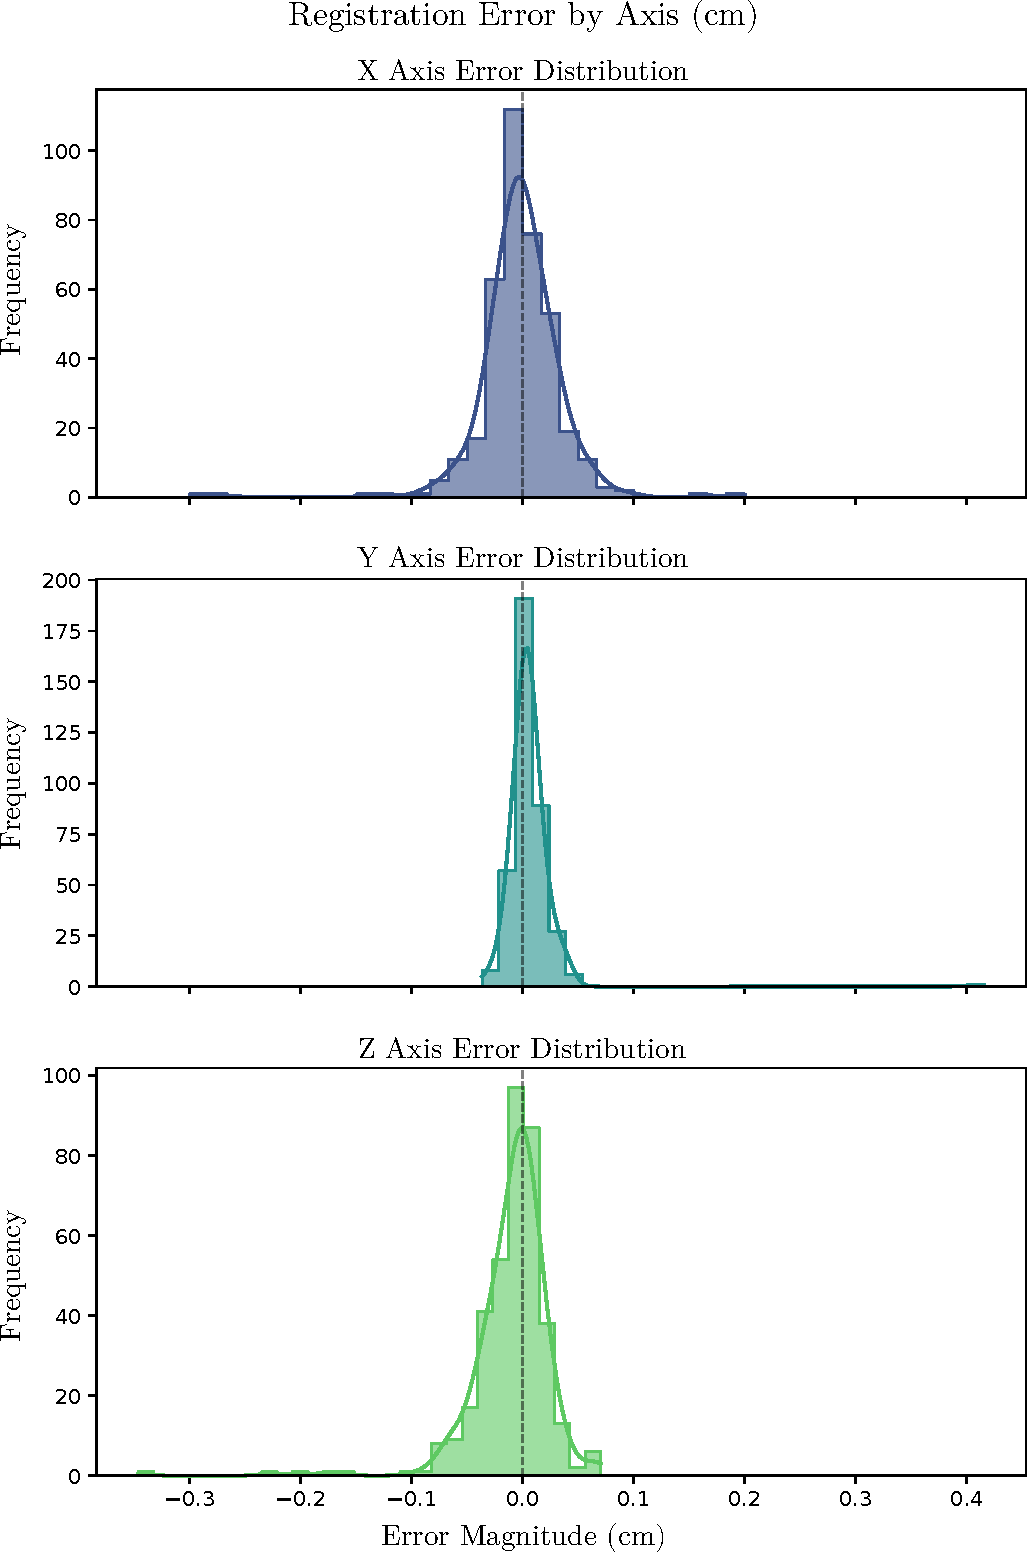
\includegraphics[width=0.4\textwidth]{figure/linear_error_hist.pdf}
    \caption{Distribution of linear error with respect to cloud solution. (Top) x error in cm. (Middle) y error in cm. (Bottom) z error in cm.}
    \label{fig:accuracy_histogram}
\end{figure}

The average error, seen in Figure \ref{fig:distance_barchart}, in the x, y, and z directions is -0.2133 cm, 0.5718 cm, and 
-1.0175 cm respectively. 
Although this shows that the algorithm is on average accurate within a cm, it is clear that there 
is a notable variance about the average for every direction. One feature of note is the lower variance in the y direction. Unity 
uses the left hand coordinate convention with the y axis facing up, so this corresponds the the axis about which the yaw values 
are being solved. It follows that this is the axis with the tightest spread in variance as it represents the roll and pitch 
locked plane ``lifting" away from corresponding point cloud plane and quickly grows in error as a solution candidate.

\begin{figure}[!htb]
    \centering
    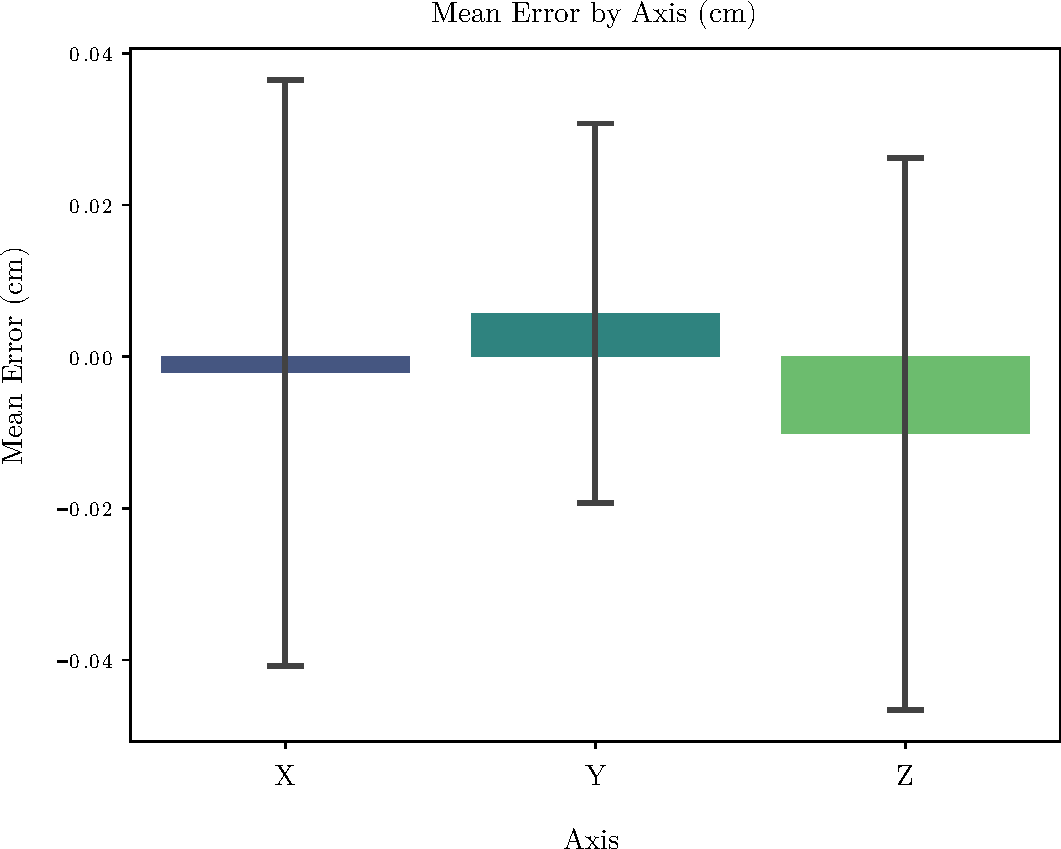
\includegraphics[width=0.4\textwidth]{figure/linear_error.pdf}
    \caption{Average linear error in each linear direction with respect to the cloud server solution.}
    \label{fig:distance_barchart}
\end{figure}

Figure \ref{fig:angle_histogram} illustrates the variation of angular accuracy resolution. Note the roll and pitch do not share the same 
x axis scale as the yaw data. This shows an extremely tight grouping when compared to yaw values due to the use of IMU gravity alignment to solve for 
roll and pitch values directly. 

\begin{figure}[!htb]
    \centering
    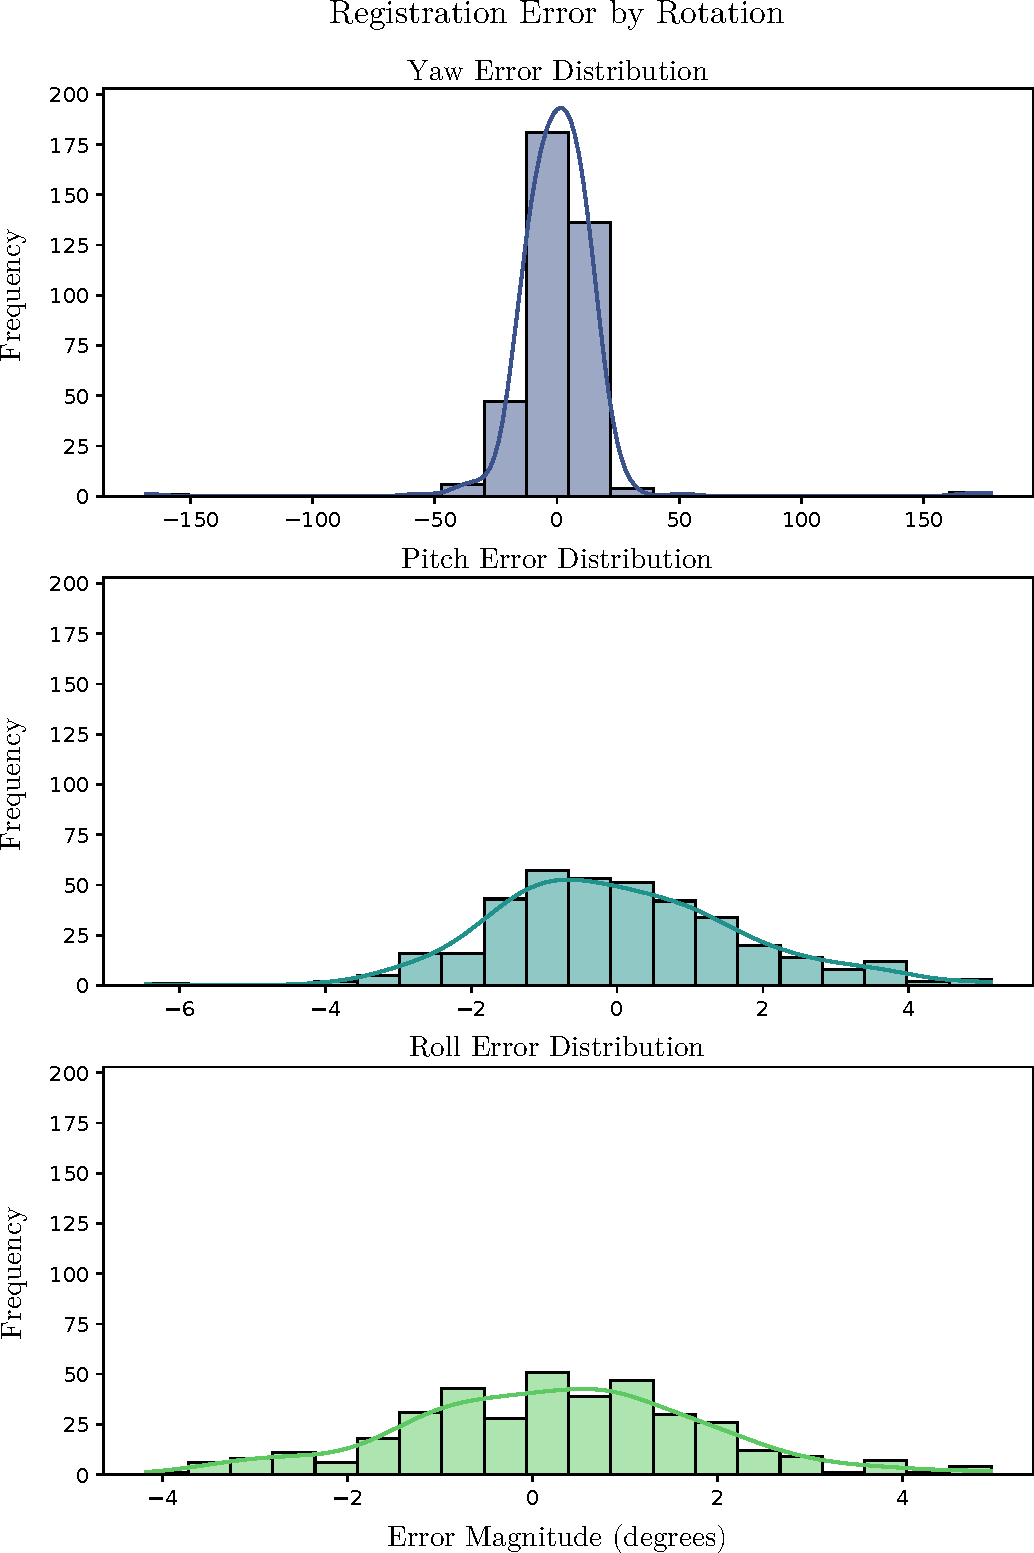
\includegraphics[width=0.4\textwidth]{figure/euler_error_hist.pdf}
    \caption{Distribution of angular error about each linear axis. (Top) Roll error in degrees. (Middle) Yaw error in degrees. (Bottom) Pitch error in degrees.}
    \label{fig:angle_histogram}
\end{figure}

Looking at the mean and standard deviation in Figure \ref{fig:angle_barchart} reveals the variance rotation accuracy 
about all three axes. As expected, roll and pitch errors are extremely small on average and do not vary greatly outside of one degree. 
In the current system we see a large variance in yaw values. With outliers in Figure \ref{fig:angle_barchart} as large as $-170^\circ$ to $170^\circ$ and values within one standard 
deviation fitting between $-19^\circ$ and $19.75^\circ$. Due to the cloud server being used as a reference point for error, there is some chance
that the roll and pitch values solved for by the peer-to-peer system are actually more accurate than the cloud based system and these errors 
are a manifestation of the limitations of the cloud-based alignment system.

\begin{figure}[htb]
    \centering
    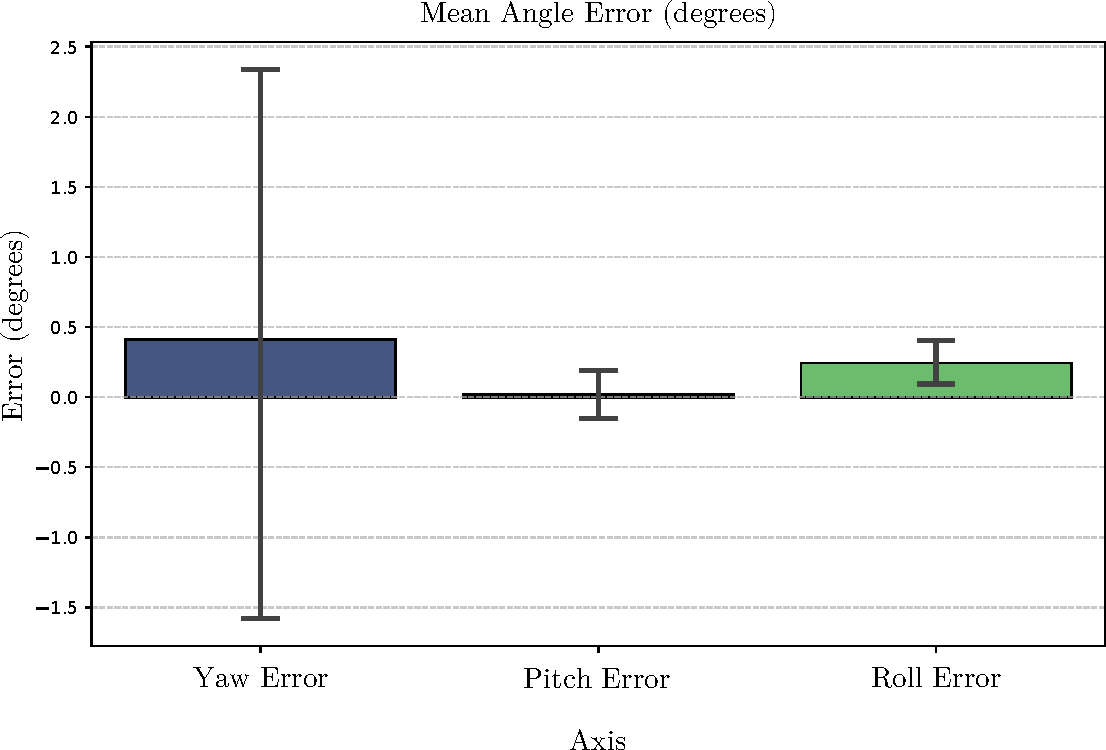
\includegraphics[width=0.4\textwidth]{figure/euler_error_bar.pdf}
    \caption{Average angular error about each axis.}
    \label{fig:angle_barchart}
\end{figure}


% \begin{table}
%     \centering
%     \begin{tabular}{ |c|c|c| }
%         \hline
%         X (m) & Y (m) & Z (m) \\
%         \hline \hline
%         0.0034 & 0.0009 & 0.0028\\
%         \hline
%     \end{tabular}
%     \caption{Standard error of alignment in all directions.}
%     \label{tab:stderror}
% \end{table}

% Figure \ref{fig:accuracy_histogram} shows the error in each direction of the user alignment solution. 

% This is due to the gravity aligned data pre-processing and indoor conditions creating 
% generally planar point clouds from floors, walls, tables, etc. Table \ref{tab:stderror} shows the standard error calculations for all directions. 
% Using our gravity constrained approach, the alignment solution is found to be accurate at the cm to sub cm level within approximately 119.69ms 
% in the testing environment.

\section{Conclusions}

From the perspective of data analysis, there are extensions to the system that would greatly enhance the 
ability to extract information from the system. First, the data collected was measured with respect to the cloud server provided 
alignment. This means that we can see how smooth the transition from peer-to-peer solution to the cloud solution may look 
for the user. Alternatively, creating an absolute reference point that would automatically place an anchor at a known world location would 
allow independent errors to be collected from both solutions. This may provide insight into where peer-to-peer solutions 
may lead to better results than cloud solutions. The second extension would be to use the transform between the world frame and 
user camera frame to transform points before conducting data analysis. The mean error in Section \ref{ExperimentalResults} may be correlated 
with the direction of the vector orthogonal to the camera plane, as cameras have less accurate tracking depth. If these were quantified in our 
system, it could be used to create a more accurate algorithm that compensates for this effect.

Future work includes further connecting the greater system design in ways that make it more 
robust to network reliability. A new user may enter the interaction that was not within the network
at the time of the initial resolve routine if the cloud server is no longer available, the user may request 
point cloud feature data from \textit{more than one} user in the group. This would allow the user to create a 
much more accurate alignment estimation than the process described above by combining the results of multiple
alignments. While this would take longer, it would serve as a better permanent anchor when there are users
available, but no cloud server. From a single user's perspective, this algorithm could be improved by 
the addition of some kind of tracked state. Once an alignment is solved for, this could be used as the beginning 
of an estimation algorithm that updates the state of the alignment rather than simply replacing it as 
the system currently does. This idea was attempted, but with no promising results in the time available. As a distributed system it would likely 
benefit the group of peers to implement this feature using multicasting for more efficient message passing between peers.

Scaling in this system is linear in most functions. AR object placement is conducted in a complete network and so a placement 
from one user to $n$ users only takes $n$ messages at most. Alignment for both peer-to-peer and cloud algorithms work the same way.
For this reason, it would be necessary to test the absolute limits of scalability using a large number of devices. Future work
would further include using docker to simulate devices sending synthetic data to test this level of scalability.

The user alignment system created here serves the purpose of reducing user-perceived end-to-end system latency. In a 
collaborative robotics scenario such as transportation, search and rescue, or our aforementioned forklift operator, 
users must be provided accurate information that they may use to plan and receive it fast enough that the information may be acted upon.
The linear scaling of this system allows any peer to become a host that may seed the alignment. This alignment may then be 
used by any number of users to send/place AR objects or information to an number of users in a decentralized fashion.
Although future work would enhance the robustness of the alignment and quantify the limits of user scaling, this work 
accomplishes feasibility for fast peer-to-peer alignment, accurate cloud alignment and user interactions are not scale limited
by system architecture.

%% if specified like this the section will be committed in review mode
% \acknowledgments{
% The authors wish to thank A, B, and C. This work was supported in part by
% a grant from XYZ.}

\clearpage


%\bibliographystyle{abbrv}
\bibliographystyle{abbrv-doi}
%\bibliographystyle{abbrv-doi-narrow}
%\bibliographystyle{abbrv-doi-hyperref}
%\bibliographystyle{abbrv-doi-hyperref-narrow}

\bibliography{references}
\end{document}
